 % ===============
\section{Analysis - TO DO}
% ===============
\label{sec:analysis}
% -------------------------------------------------------------
\subsection{Validator duty selection}
% ------------------------------------------------------------
The selection of validators to be part of committees or to be selected as a proposer needs to be done in an unpredictable, or random, way to ensure that the selection cannot be manipulated by bad actors.

However, in a blockchain system, all nodes need to come to consensus, and the key ``randomness lever'' is the seed used in the  calculation that would have the same outcome for all nodes. Therefore the seed needs to be unpredictable \cite{buterin2020}.



In the Consensus Layer there are a few different approaches to achieve randomness used in selection of validators for duties:
\begin{itemize}
\item Aggregators are selected via a \gls{vrf} lottery \cite{Edgington2023}.
\end{itemize}


% ------------------------------------------------
\subsubsection*{Proposer}
% ------------------------------------------------
Endianness, the order of bytes in the binary representation of a number, is not commonly of interest, but in the case of index shuffling and proposer selection, the RANDAO, and serialising with SSZ, the endianness does matter. Initially big-endian was used, i.e. the first byte is the most-significant byte, but this has now changed mainly to little-endian, i.e. the first byte is the least-significant byte \cite{Edgington2023}.

% From. Ben's book: https://eth2book.info/capella/part3/helper/misc/#compute_proposer_index

% Mike Neuder links to the compute_proposer_index method: https://github.com/ethereum/consensus-specs/blob/9c35b7384e78da643f51f9936c578da7d04db698/specs/phase0/beacon-chain.md#compute_proposer_index 
% in his "Increase the MAX_EFFECTIVE_BALANCE – a modest proposal" blog: https://ethresear.ch/t/increase-the-max-effective-balance-a-modest-proposal/15801


The \textit{swap-or-not-shuffle} technique \cite{hoang2014}  is used to shuffle the validator indices in preparation for the selection of a block proposer. This is done in \href{https://github.com/ethereum/consensus-specs/blob/9c35b7384e78da643f51f9936c578da7d04db698/specs/phase0/beacon-chain.md#compute_shuffled_index}{\textit{compute\_shuffled\_index}}.

\href{https://notes.ethereum.org/@vbuterin/Sys3GLJbD}{Vitalik's annotated spec} explains the reasoning behind the process of computing the proposer index. ``The idea is that it chooses a proposer, accepts them with BALANCE/32 probability, and if it fails it keeps trying. This is done so that the probability of being selected as a proposer remains proportional to balance.''

The computation to determine the proposer for the next block is done in \href{https://github.com/ethereum/consensus-specs/blob/9c35b7384e78da643f51f9936c578da7d04db698/specs/phase0/beacon-chain.md#compute_proposer_index}{\textit{compute\_proposer\_index}}: 

\lstset{language=Python}

\begin{lstlisting}
def compute_proposer_index(state: BeaconState, indices: Sequence[ValidatorIndex], seed: Bytes32) -> ValidatorIndex:
    """
    Return from ``indices'' a random index sampled by effective balance.
    """
    assert len(indices) > 0
    MAX_RANDOM_BYTE = 2**8 - 1
    i = uint64(0)
    total = uint64(len(indices))
    while True:
        candidate_index = indices[compute_shuffled_index(i % total, total, seed)]
        random_byte = hash(seed + uint_to_bytes(uint64(i // 32)))[i % 32]
        effective_balance = state.validators[candidate_index].effective_balance
        if effective_balance * MAX_RANDOM_BYTE >= MAX_EFFECTIVE_BALANCE * random_byte:
            return candidate_index
        i += 1
\end{lstlisting}


Therefore, we iterate through the shuffled indices, starting with the first entry and then check whether it passes the selection criteria. If it doesn't, then the next candidate index goes through the same checks.

The validator's effective balance is multiplied by 255 and then compared to the product of the generated \textit{random\_byte}, which we assume is uniformly randomly distributed across 0 to 255,  and the \textit{MAX\_EFFECTIVE\_BALANCE} which is now 2,048 ETH. 

Therefore the probability of a validator being the proposer if their index was selected from the list can be calculated as follows:
% , as indicated by Neuder in his \href{https://ethresear.ch/t/increase-the-max-effective-balance-a-modest-proposal/15801}{blog post} 

%We already weight the probability of becoming a proposer by the effective balance of that validator. See compute\_proposer\_index 17. Currently, if a validator’s effective balance (EB) is below the MaxEB, they are selected as the proposer given their validator index was randomly chosen only if,
\begin{equation}
\label{eqn:1}
\begin{split}
& P(proposer) = P(EB * 255 \geqslant MaxEB*r) \texttt{ } where \texttt{ } r \sim U(0,255), \textit{ } r = random\_byte, EB = \textit{validator effective balance} \\
& \therefore P(proposer) = P\left(r \leqslant \frac{255*EB}{MaxEB} \right) \\
& \therefore \textit{if } EB = MaxEB \implies P(proposer) = 1\\
\end{split}
\end{equation}
%
Therefore, if the effective balance of the candidate validator equalled the maximum effective balance, then the validator becomes the proposer with probability 1. 

This creates some interesting scenarios when the maximum effective balance is increased to 2,048 ETH. As before, a fully consolidated validator will become a proposer with a probability of 1 if the 
validator's index was randomly selected as the next candidate. 

\begin{equation*}
\begin{split}
& \textit{Given the candidate index belongs to a solo staker with an effective balance of 32 ETH, then } \\
& P(proposer \texttt{ } check \texttt{ } passed) = P\left(r \leqslant \frac{255*32}{2048} \right) = P(r \leqslant 3.98) = \left(\frac{3.98-0}{255}\right) = 0.016\\
& \therefore P(proposer \texttt{ } check \texttt{ } passed)  \equiv \left(\frac{32}{2048}\right) = 0.016 \\
& \\
& \therefore \textit{Given the candidate index belongs to a staker with a partially consolidated validator (2 * 32 ETH) EB , then } \\
&  P(proposer \texttt{ } check \texttt{ } passed) = \left(\frac{64}{2048} \right) = 0.031\\
& \\
& \therefore \textit{Given the candidate index belongs to a staker with a partially consolidated validator (5 * 32 ETH) EB , then } \\
& P(proposer \texttt{ } check \texttt{ } passed) = \left(\frac{160}{2048} \right) = 0.078\\
\end{split}
\end{equation*}

\begin{figure}[htbp]
\begin{center}
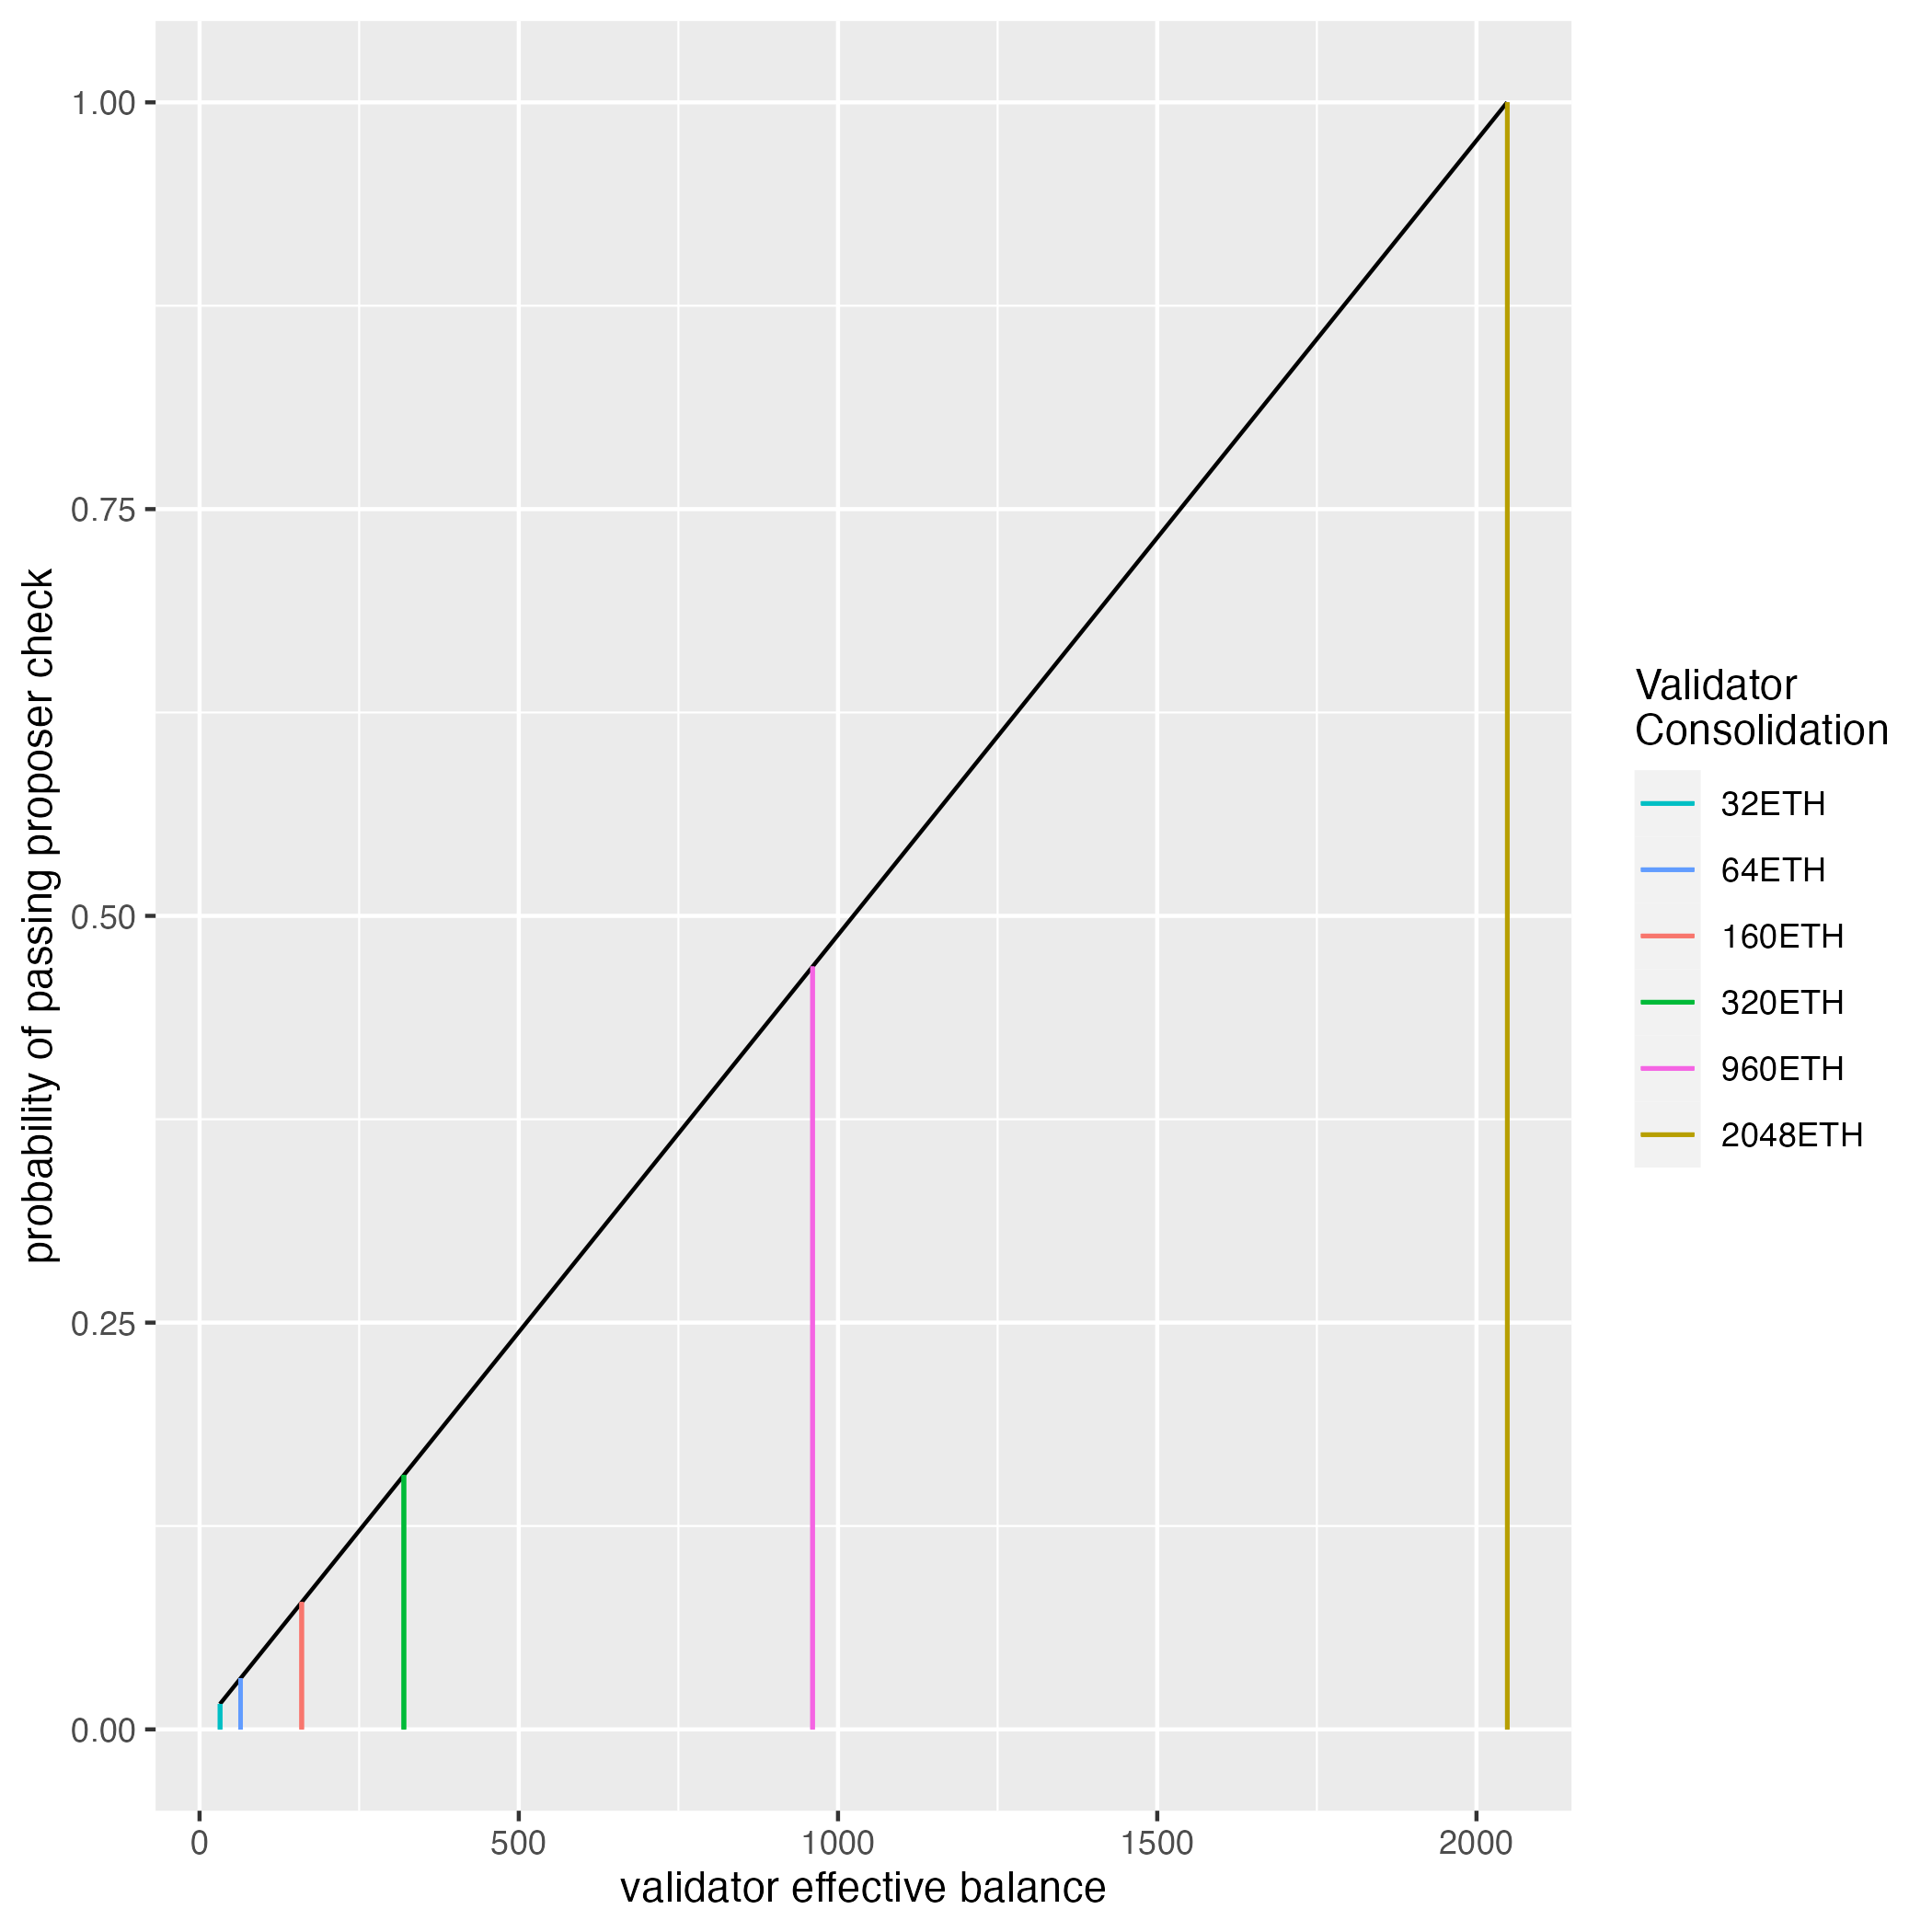
\includegraphics[width=0.6\linewidth]{images/proposer_check_graph}
\caption{Probability of passing the proposer eligibility check for a candidate validator with an EB ranging from 32 to 2,048 ETH}
\label{fig:proposerEB}
\end{center}
\end{figure}

In other words, the probability of passing the check for selection to propose the next block varies from 0.016 for an unconsolidated validator to 1 for a fully consolidated validator, if that validator’s index is selected as the next candidate.

Assuming a validator set size of 716,800, then
the probability of any validator being chosen as the candidate index for the next block proposer is: \\
$P(candidate) = \frac{1}{(Active \texttt{ } validator \texttt{ } set \texttt{ } size)} = \frac{1}{ 716,800} = 0.000001395$, or 0.0001395 \%. 

Previously, providing a validator maintained its effect balance at 32 ETH, once its index was selected as the next candidate, it would have passed the proposer selection test with certainty (probability of 1, i.e. 100\%).

Putting it another way:
\begin{equation*}
\begin{split}
& \textit{Given EB=32 ETH, then currently } \\
& P(candidate \& proposer) = P(candidate) * P(proposer) = 0.000001395 * 1 = 0.000001395 \\
& \textit{After MaxEB = 2048 ETH, this changes to:} \\
& P(candidate \& proposer) = 0.000001395 * 0.016 = 0.00000002232 \\
\end{split}
\end{equation*}

Let us look at some example scenarios, assuming an active validator set of 716,800 validators, i.e. a total deposit size of $716,800 * 32 ETH \approx 22.94$ \textit{M ETH}:
\begin{enumerate}
\item Validator set comprises only validators with an effective balance of 32 ETH.
\item Validator set comprises only validators that are fully consolidated, i.e. each validator has an effective balance of 2,048 ETH.
\item Validator set comprises a combination of validators: solo stakers, partially consolidated stakers and fully consolidated stakers.
\end{enumerate}

Interesting questions:
\begin{itemize}
\item What is the probability that no proposer is selected for a slot when no consolidation has yet happened? This situation could occur during implementation time, before stakers merge some or all of their validators.
\end{itemize}


\noindent
\textbf{\textit{Scenario 1}} \\
% -------------------
\noindent
In figure \ref{fig:random} on page \pageref{fig:random} we generated 716,800 random values from \textit{U(0,255)} \\

\begin{figure}[htbp]
\begin{center}
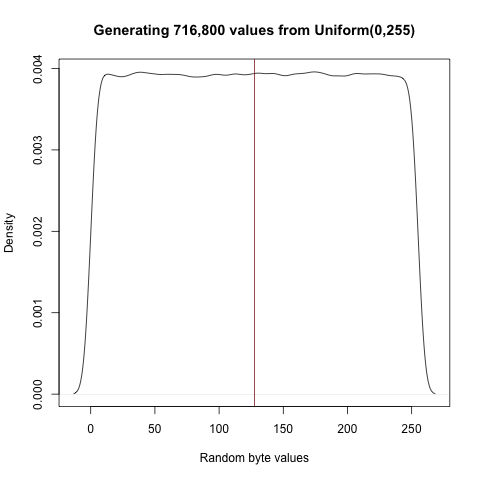
\includegraphics[width=0.5\linewidth]{images/validator-indices-density}
\caption{Distribution of 716,800 random bytes generated from U(0,255)}
\label{fig:random}
\end{center}
\end{figure}


\begin{figure}[htbp]
\begin{center}
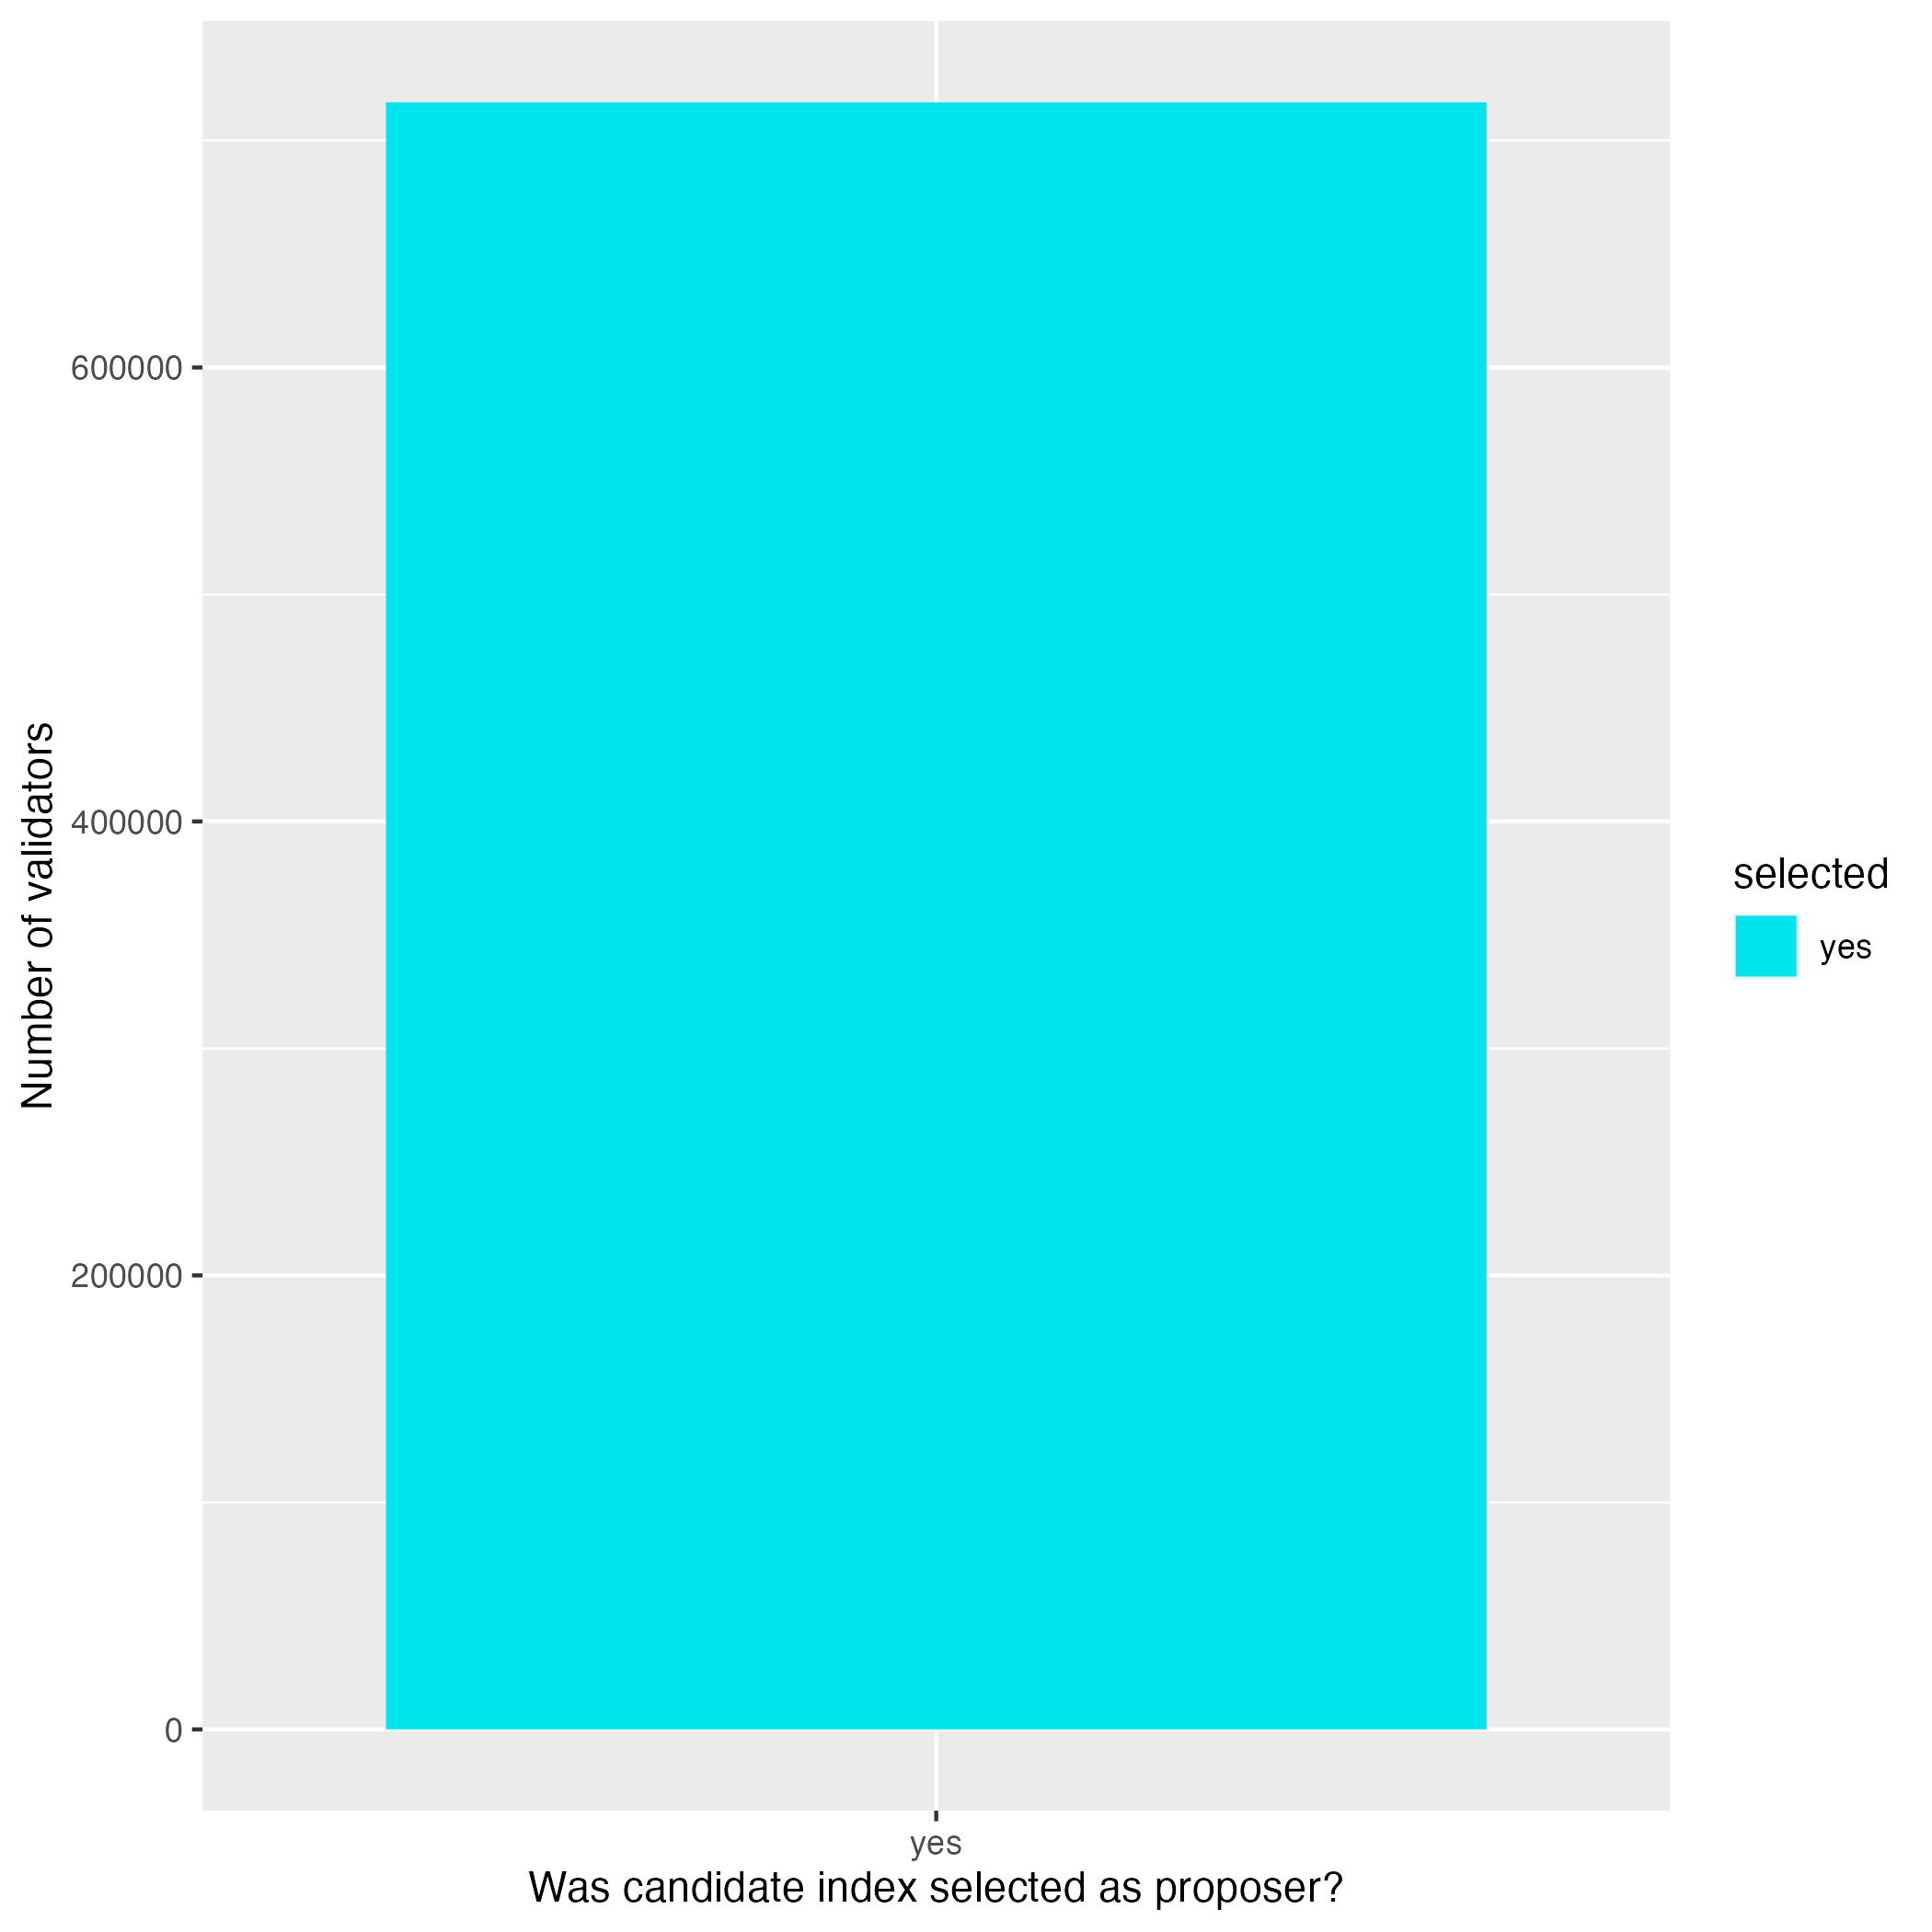
\includegraphics[width=0.45\linewidth]{images/current-solo-barchart}
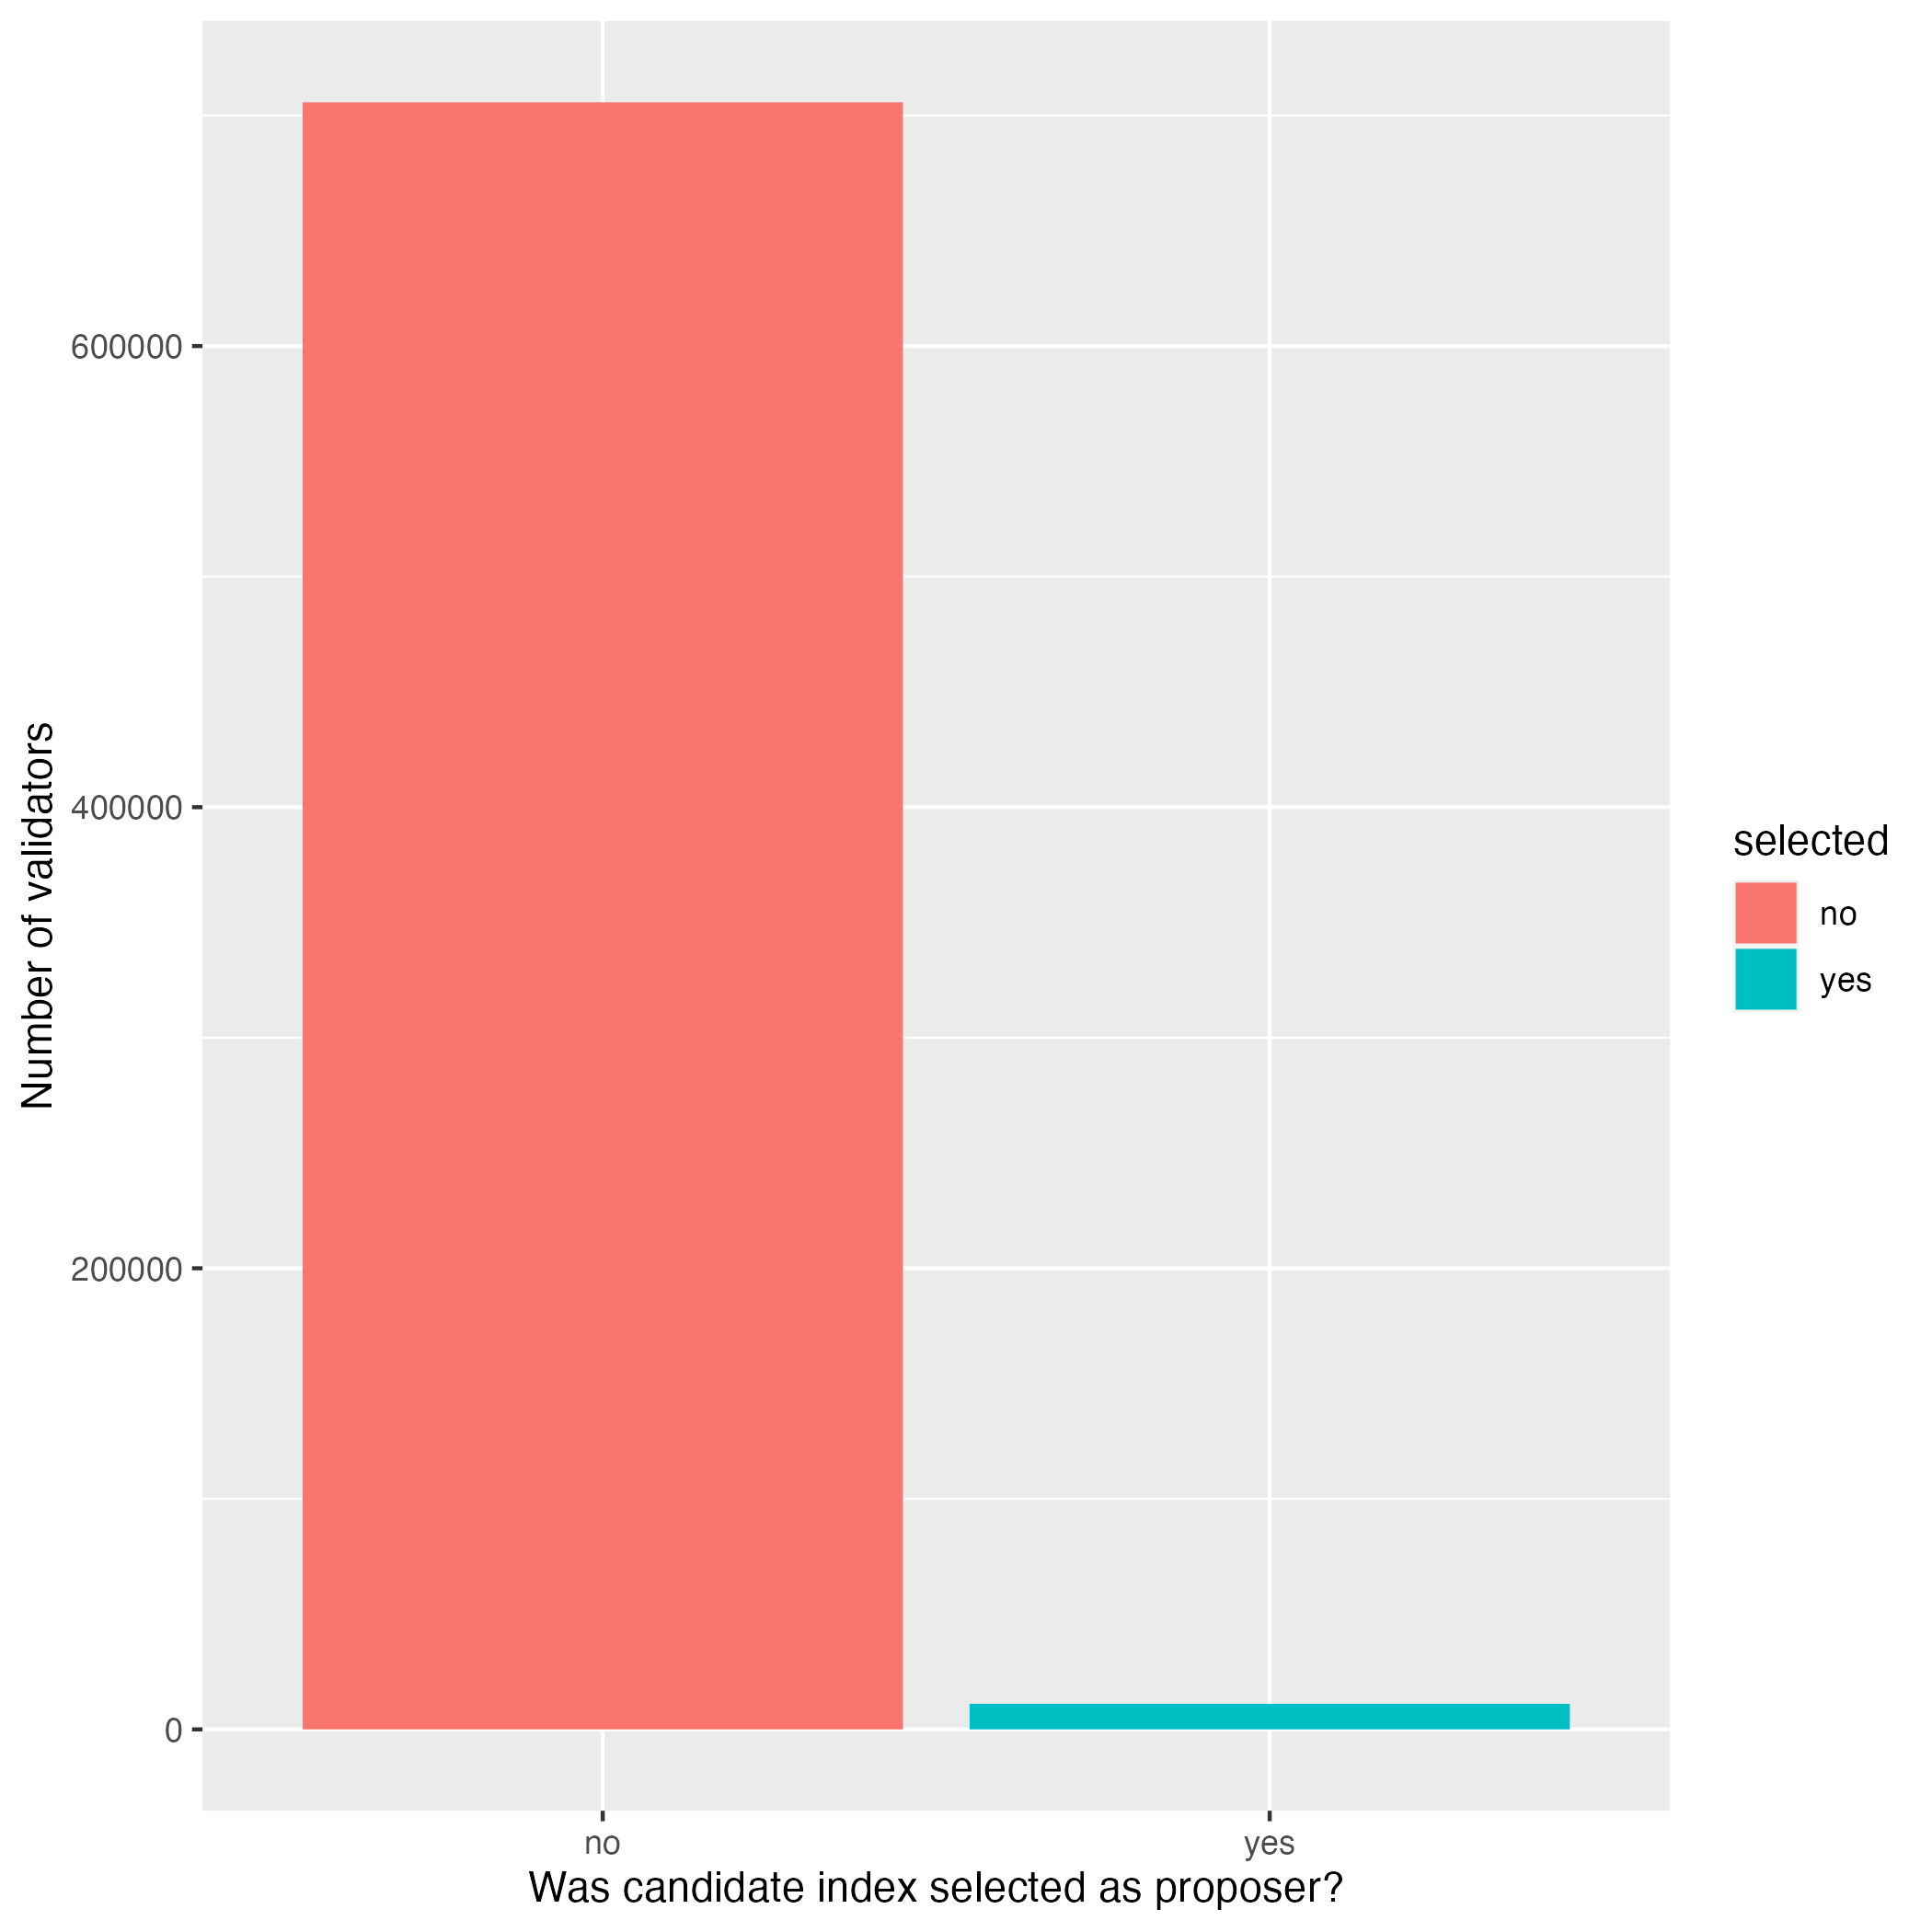
\includegraphics[width=0.45\linewidth]{images/maxeb-solo-barchart} \\
(a) \hspace{180pt}     (b)
\caption{Proportion of validators with random byte that passes proposer check if all validators have 32 ETH effective balance, and (a) maxEB = 32 ETH, (b) maxEB = 2,048 ETH}
\label{fig:maxebsolo}
\end{center}
\end{figure}

\noindent
\textbf{\textit{Scenario 2}} \\
% -------------------
\noindent
In this scenario we have full consolidation by all stakers, so probabilities and mechanisms for selection remain unchanged, i.e. when a candidate validator's balance = maxEB, then they will be selected with certainty, i.e. a probability of 1. \\

\clearpage
\noindent
\textbf{\textit{Scenario 3}} \\
% -------------------
\noindent
A more interesting scenario is when we look at a variety of effective balances. As an example, let us assume that the validator set of 716,800 validators is made up of a combination of consolidation options as shown in Table \ref{tbl:scenario3} on page \pageref{tbl:scenario3}. Based on this chosen configuration, the total validator set size reduces to 297,248: \\

\noindent
\textit{Number of single validators} $= \frac{716,800 * 0.30}{1} = 215,040 $ \\
\textit{Number of 64ETH validators} $= \frac{716,800 * 0.20}{2} = 71,680 $ \\
\textit{Number of 320ETH validators} $= \frac{716,800 * 0.10}{10} = 7,168 $ \\
\textit{Number of 2,048ETH validators} $= \frac{716,800 * 0.30}{64} = 3,360 $ \\
\textit{Adjusted validator set after consolidation}$ = 215,040 + 71,680 + 7,168 + 3,360 = 297,248$ \\

\noindent
 We calculate the probability that a validator is selected and passes the check for proposer eligibility, as the product of the probability of being the candidate index  and the probability of passing the proposer check, since these two events are independent, i.e. $P(A \cap B) = P(A/B)P(B) = P(A)P(B)$. Using the logic from equation \ref{eqn:1} and the example calculations that followed, we populated the table accordingly.
\begingroup
\renewcommand{\arraystretch}{1.5} % Default value: 1
\begin{table}[htp]
\caption{Active validator set composition for Scenario 3}
\label{tbl:scenario3}
\begin{center}
\begin{tabular}{|c|c|c|c|c|c|}
\hline
\textbf{Staker} & \textbf{\% of total} & \textbf{Effective} & \textbf{P(candidate)} & \textbf{P(proposer} & \textbf{P(candidate} \\
\textbf{Consolidation} & \textbf{deposit } & \textbf{balance} &\textbf{ } & \textbf{check = Y) } & \textbf{ \& selected)} \\
\hline
Single & 30\% & 32 ETH & $\frac{215,040}{297,248} = 0.723$ & 0.016 & $0.723*0.016 = 0.0116$\\
Partial (2-fold) & 20\% & 64 ETH & $\frac{71,680}{297,248} = 0.241$ & 0.031 & $0.241*0.031 = 0.0075$\\
Partial (10-fold) & 10\% & 320 ETH & $\frac{7,168}{297,248} = 0.024$ & 0.156 & $0.024*0.156 = 0.0037$\\
Fully (64-fold) & 30\% & 2,048 ETH & $\frac{3,360}{297,248} = 0.011$ & 1.000 & 0.0113*1.000 = 0.0113 \\
\hline
TOTAL & 100\% & \texttt{ } & 1.00 & \texttt{ } &  \texttt{ } \\
\hline

\end{tabular}
\end{center}
\end{table}%
\endgroup

The above scenario tells an interesting story. If the lion share of the total stake is shared equally between single and fully consolidated validators, then it is approximately equally likely for either category to be selected as a proposer of the next block. The varying proportions of, and extent of, consolidation would appear to be less desirable, but we need to put these observations in the context of the total stake for each of the categories in the scenario. \\

Taking a very simple example, say we have a validator set size of 100, where 32 validators are run by single stakers, and there is 1 large staker running 64 validators. The large staker decides to consolidate all 64 validators into one `super' validator. Then the probability of the large staker's validator being selected as the candidate index for proposing the next block is $\frac{1}{33} = 0.03$, where previously it would have been $\frac{64}{100} = 0.64$ that one of its validators would be the candidate index selected. Once the check for proposer eligibility is made, the super validator will always pass that check, i.e. probability of 1. For a solo validator to be the selected candidate index would also be 0.03, but the probability that one of the solo stakers is selected, rather than a super validators is $\frac{32}{33} = 0.97$.

\noindent
\clearpage
\noindent
The probability that no validator in the active validator set is selected as proposer immediately following the switch to the new maximum effective balance EIP-7251, can be calculated as follows:\\

We know that if a candidate did not pass the selection process, then the next one in the shuffled index is used to check if they pass the proposer eligibility check. 

Therefore we are interested in the probability that every  validator in the active validator set failed the eligibility check.

We know that prior to consolidation, all the validators will have an \gls{eb} of 32 ETH.\\
$\therefore$ \textit{ P(no proposer selected) =} $\binom{n}{k} p^k q^{(n-k)} = \binom{716,800}{716,800} 0.984^{716,800}0.016^0 = (0.984)^{716,800}$\\
%Alternatively, $1 - \textit{P(one proposer selected)}$  = 
$\therefore$ \textit{ P(no proposer selected) = } $0.984^{716,800} = 0$ \\
Although for each validator the probability of passing the proposer check is quite low, viz. 0.016, it is highly unlikely, and essentially impossible, for every single validator in the validator set to fail the selection test.\\

The probability of selecting the first candidate = 1/n, the probability of the next is 1/(n-1) .... 1/1 = $ \frac{1}{716,800!}$

\noindent
\textbf{\textit{Proposer selection \gls{bn}}} \\
% -------------------
\noindent
Building on Scenario 3, we can develop a simple Bayesian network (BN)  to explore the consequences of various choices. The total number of validators before any consolidation of stake is assumed to be 716,800.  Moreover, we will make some assumptions about a possible distribution of consolidated and single validators for various categories of staker. All these assumptions can be replaced with alternative assumptions in the BN. 

The diagram in Figure \ref{fig:proposer} on page \pageref{fig:proposer} is visual representation of the example scenario depicted in the \gls{bn}.

\begin{figure}[htbp]
\begin{center}
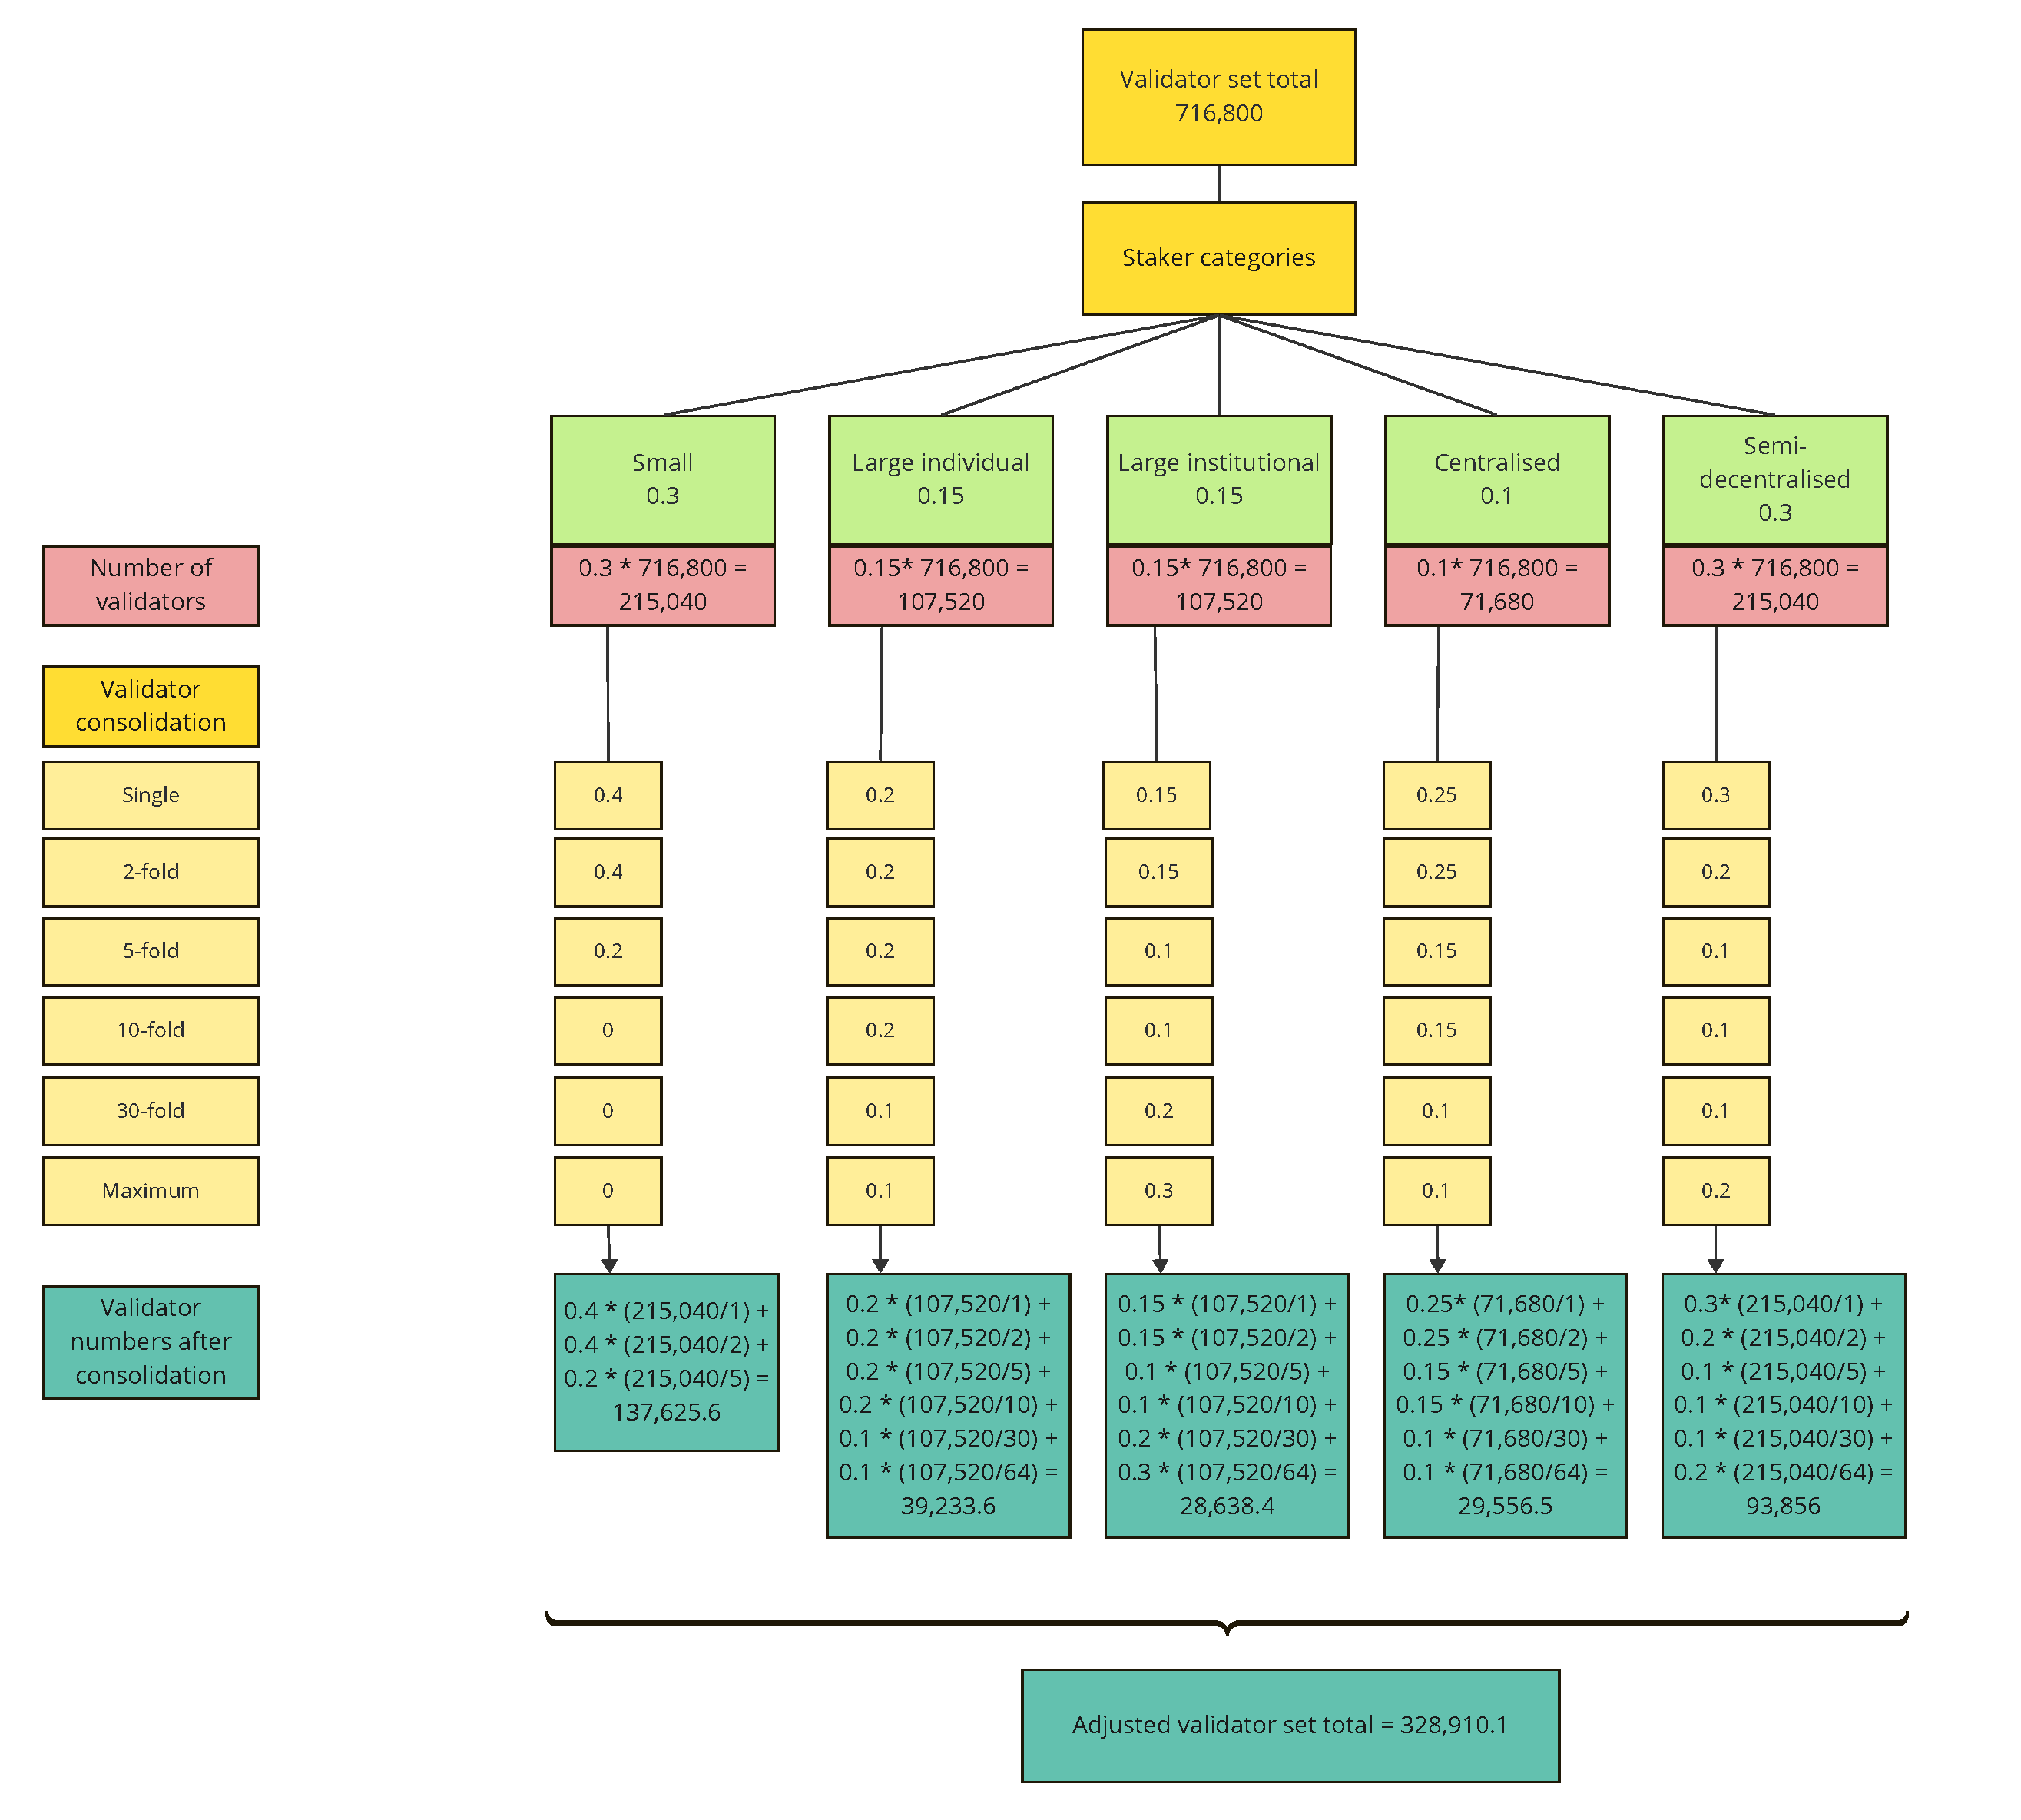
\includegraphics[width=\linewidth]{images/proposer-selection-diagram.pdf}
\caption{Visual representation of the example scenario for validator consolidation}
\label{fig:proposer}
\end{center}
\end{figure}


The following tables describe the key factors (nodes) in the BN and the \gls{npt} attached to each node. Figures \ref{fig:proposerbn} and \ref{fig:proposerbnrun} depict the BN structure and the resulting marginal probabilities when we run the network, respectively.
 
\begin{figure}[htbp]
\begin{center}
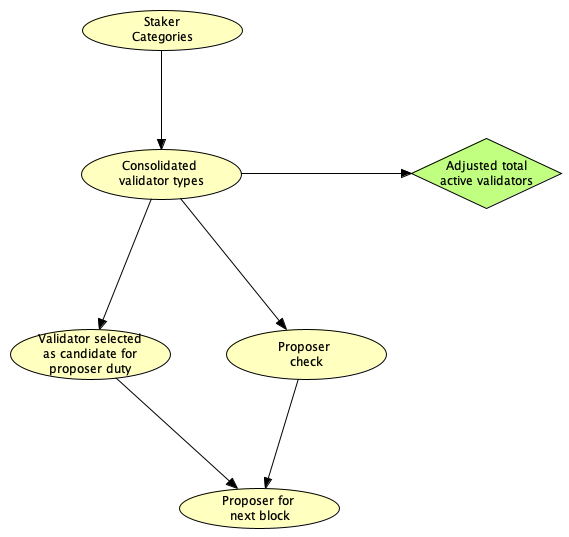
\includegraphics[width=0.6\linewidth]{images/proposer-bn}
\caption{BN for proposer selection after EIP-7251}
\label{fig:proposerbn}
\end{center}
\end{figure}

\begin{figure}[htbp]
\begin{center}
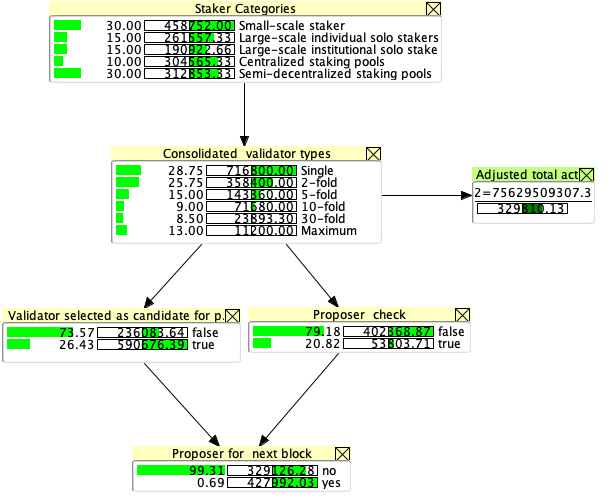
\includegraphics[width=0.7\linewidth]{images/proposer-bn-run}
\caption{Running the proposer selection BN}
\label{fig:proposerbnrun}
\end{center}
\end{figure}

\clearpage

 \begin{table}[htp]
\caption{Staker categories - \gls{npt}}
\begin{center}
\begin{tabular}{|l|l|c|}
\hline
\textbf{Category} & \textbf{Description} & \textbf{Fraction of} \\
 & & \textbf{validator set} \\
 \hline
Small-scale solo stakers & 32 - a few hundred ETH & 0.30 \\
Large-scale individual solo stakers & 1000+ ETH & 0.15 \\
Large-scale institutional solo stakers & companies staking their own ETH & 0.15 \\
Centralized staking pools & & 0.10 \\
Semi-decentralized staking pools & Rocketpool, Lido... each one is different & 0.30 \\
\hline
\end{tabular}
\end{center}
\label{tbl:stakers}
\end{table}%

\begin{table}[htp]
\caption{Consolidated validator types - \gls{cpt}}
\begin{center}
\begin{tabular}{|l|c|c|c|c|c|}
\hline
& \multicolumn{5}{c|}{\textbf{Staker categories}} \\
\cline{2-6}
\textbf{Validator}       & Small-scale & Large-scale & Large-scale & Centralised  & Semi- \\
\textbf{consolidation} & staker         & individual    & institutional  & staking pools& decentralised \\
                                  &                    & staker          & staker         &                      & staking pools \\
\hline
 Single  & 0.4	& 0.2	 & 0.15 & 0.25 & 0.3 \\
 2-fold  & 0.4 & 0.2 & 0.15 & 0.25 & 0.2 \\
 5-fold  & 0.2	 & 0.2 & 0.1 & 0.15 & 0.1 \\
 10-fold & 0 & 0.2 & 0.1 & 0.15 & 0.1 \\
 30-fold  & 0 & 0.1 & 0.2 & 0.1 & 0.1 \\
 Maximum & 0 & 0.1 & 0.3 & 0.1 & 0.2 \\
\hline
\end{tabular}
\end{center}
\label{tbl:consolidation}
\end{table}%

\begin{table}[htp]
\caption{Proposer check - \gls{cpt}}
\begin{center}
\begin{tabular}{|l|c|c|c|c|c|c|}
\hline
& \multicolumn{6}{c|}{\textbf{Validator consolidation}} \\
\cline{2-7}
\textbf{Proposer}  & Single & 2-fold & 5-fold & 10-fold  & 30-fold & Maximum \\
\textbf{check passed}       &            &           &           &              &              & \\
\hline
false  & 0.984375 & 0.96875 & 0.921875 &0.84375 & 0.53125 & 0.0 \\
 true  & 0.015625 & 0.03125 & 0.078125 &0.15625 & 0.46875 & 1.0 \\
 \hline
\end{tabular}
\end{center}
\label{tbl:proposercheck}
\end{table}%


\begingroup
\renewcommand{\arraystretch}{1.5} % Default value: 1
\begin{table}[htp]
\caption{P(validator selected as candidate proposer)}
\label{tbl:candidate}
\begin{center}
\begin{tabular}{|c|c|c|c|}
\hline
\textbf{Validator} & \textbf{Marginal} & \textbf{Number of} & \textbf{P(selected as} \\
\textbf{consolidation} & \textbf{probability } & \textbf{validators} &\textbf{ candidate)}  \\
\hline
Single & 28.75\% & $\frac{0.2875 * 716,800}{1} = 206,080$ & $\frac{206,080}{329,810} = 0.6248$ \\
Partial (2-fold) & 25.75\% &  $\frac{0.2575 * 716,800}{2} = 92,288$ & $\frac{92,288}{329,810} = 0.2798$ \\
Partial (5-fold) & 15.00\% &  $\frac{0.1500 * 716,800}{5} =  21,504$ & $\frac{21,504}{329,810} =  0.0652$ \\
%Partial (10-fold) & 9.00\% &  $\frac{0.0900 * 716,800}{10} = 6,451.2$ & $\frac{6,451.2}{329,810} = 0.0196$ \\
Partial (10-fold) & 9.00\% &  $\frac{0.0900 * 716,800}{10} = 6,451$ & $\frac{6,451}{329,810} = 0.0196$ \\
%Partial (30-fold) & 8.50\% &  $\frac{0.0850 * 716,800}{30} = 2,030.93$ & $\frac{2,030.93}{329,810} = 0.0062$ \\
Partial (30-fold) & 8.50\% &  $\frac{0.0850 * 716,800}{30} = 2,031$ & $\frac{2,031}{329,810} = 0.0062$ \\
Fully (64-fold) & 13.00\% &  $\frac{0.1300 * 716,800}{2,048} = 1,456 $ & $\frac{1,456}{329,810} =  0.0044$\\
\hline
TOTAL & 100\% & 329,810 & 1.0000 \\
\hline

\end{tabular}
\end{center}
\end{table}%
\endgroup

Note that the probability that any one validator in the heterogeneous validator set is selected is $\frac{1}{329,810} = 0.000003$, but the probability that the validator belongs to a certain `type' of validator differs as shown in Table \ref{tbl:candidate}. Similarly, the probability that a validator from a particular staker is selected as the candidate index is proportional to the number of validators in the active validator set, regardless of whether it is consolidated or not.

\clearpage
% ------------------------------------------------
\subsubsection*{Sync committee}
% ------------------------------------------------
As discussed in the \href{https://ethresear.ch/t/increase-the-max-effective-balance-a-modest-proposal/15801/3}{blog post}, the expectation is that this selection process will work as designed even when there is a large increase in Max\gls{eb} \cite{Neuder2023a}.

Sync committee members are selected with replacement from the active validator set. The probability of being selected is proportional to the ratio of the validator's effective balance, i.e. the number of increments, \textit{n}, to the total number of increments in the validator set, \textit{T}, i.e. $\frac{n}{T}$ \cite{Edgington2023}. 

The denominator for the acceptance probability is MaxEB which means the probability will change from $\frac{b}{32}$ to $\frac{b}{2,048}$, where \textit{b = validator effective balance}. Check whether this adversely affects validators with a small stake, apart from the expected increase in time to select the committee, as D'Amato and Neuder pointed out \cite{damato2023}.

From the \href{https://github.com/ethereum/consensus-specs/pull/2130#discussion\_r532499943}{discussion in Github} it is interesting to note that it was a deliberate choice to select sync committee members \textbf{with replacement}. This strategy is necessary if there is a situation where the number of active validators is less than pre-determined sync committee size. 

Therefore, theoretically a validator can be chosen more than once to be in the committee, and consequently we can conclude that the size of the next sync committee is always $\leqslant SYNC\_COMMITTEE\_SIZE$.  

The committee selection process is handled in \href{https://eth2book.info/capella/part3/helper/accessors/#def\_get\_next\_sync\_committee\_indices}{\textit{get\_next\_sync\_committee\_indices}} \cite{Edgington2023} shown below: 

\lstset{language=Python}

\begin{lstlisting}
def get_next_sync_committee_indices(state: BeaconState) -> Sequence[ValidatorIndex]:
    """
    Return the sync committee indices, with possible duplicates, for the next sync committee.
    """
    epoch = Epoch(get_current_epoch(state) + 1)

    MAX_RANDOM_BYTE = 2**8 - 1
    active_validator_indices = get_active_validator_indices(state, epoch)
    active_validator_count = uint64(len(active_validator_indices))
    seed = get_seed(state, epoch, DOMAIN_SYNC_COMMITTEE)
    i = 0
    sync_committee_indices: List[ValidatorIndex] = []
    while len(sync_committee_indices) < SYNC_COMMITTEE_SIZE:
        shuffled_index = compute_shuffled_index(uint64(i % active_validator_count), active_validator_count, seed)
        candidate_index = active_validator_indices[shuffled_index]
        random_byte = hash(seed + uint_to_bytes(uint64(i // 32)))[i % 32]
        effective_balance = state.validators[candidate_index].effective_balance
        if effective_balance * MAX_RANDOM_BYTE >= MAX_EFFECTIVE_BALANCE * random_byte:
            sync_committee_indices.append(candidate_index)
        i += 1
    return sync_committee_indices
  \end{lstlisting}  
  
  \noindent 
 Currently: \\
 \noindent   
$SYNC\_COMMITTEE\_SIZE = 2^9 = 512$ \textit{ validators}\\
$EPOCHS\_PER\_SYNC\_COMMITTEE\_PERIOD = 2^8 = 256$ \textit{ epochs}, which is $\approx 27 hours$, i.e. sync committees are roughly in place for a day before the next committee takes over.
 
The decision to accept a selected candidate validator  to participate in the sync committee, follows the same logic as is used for the acceptance of the candidate validator as a proposer. However, in this instance, we continue with the process until we have 255 sync committee members, which may contain duplicates as mentioned previously.
 
To demonstrate that this process works as intended we consider a couple of simple example scenarios:
\begin{enumerate}
\item The active validator set has fewer than 255 validators
\item The active validator set has more than 255 validators
\end{enumerate}

The first case is currently very unrealistic with an active validator count of approximately 900,000 at the end of January 2024, but we have left it in for completeness.


\begin{table}[htp]
\caption{Simple sync committee example scenario 2 - more than 255 validators}
\begin{center}
\begin{tabular}{|l|c|c|c|c|c|c|r|}
\hline
& \textbf{Before } & \multicolumn{6}{c|}{\textbf{After}} \\
& \textbf{consolidation} & \multicolumn{6}{c|} {\textbf{ consolidation}} \\
\cline{2-8}
\textbf{Staker}  & Single & Single & 2-fold & 5-fold & 10-fold & Maximum & Total \\
\hline
A & 128 & 128 & 0 &0 & 0 & 0 & 128 \\
B  & 128 & 0 & 0 &0 & 0 & 2 & 2 \\
C  & 128 & 14 & 5 & 4 & 2 & 1 & 26\\
 \hline
 TOTAL & 384 & 142 & 5 & 4 & 2 & 3 & 156 \\
 \hline
\end{tabular}
\end{center}
\label{tbl:syncscenario}
\end{table}%

Note that we consider a consolidated validator as consisting of one or more virtual validators.
Assuming that ``After consolidation'' in Table \ref{tbl:syncscenario} represents the decisions made by each of the stakers regarding the validators they run after the implementation of EIP-7521. We can calculate the probabilities prior to and after EIP-7521 for each of these three staker groups. Staker group A consists of single stakers, group B of consolidating into 10-fold and maxEB validators and group B has a collection of various degrees of consolidated validators. Table \ref{tbl:syncprobs} summarises the various probabilities for sync committee membership.

\begin{table}[htp]
\caption{Sync committee probabilities for example scenario }
\begin{center}
\begin{tabular}{|l|c|c|c|c|c|c|c|c|c|c|c|c|}
\hline
& \multicolumn{2}{c|}{\textbf{Before }} & \multicolumn{8}{c|}{\textbf{After}} \\
& \multicolumn{2}{c|}{\textbf{EIP-7251}} & \multicolumn{8}{c|}{\textbf{EIP-7521}} \\
\cline{2-3} \cline{4-11} 
& \multicolumn{2}{c|}{Single} &  \multicolumn{2}{c|}{Single} & \multicolumn{2}{c|}{5-fold} &  \multicolumn{2}{c|}{10-fold} &  \multicolumn{2}{c|}{Maximum} \\
\cline{2-3} \cline{4-5} \cline{6-7} \cline{8-9} \cline{10-11}
 & Prob &  Prob  & Prob &  Prob  & Prob &  Prob & Prob &  Prob  & Prob &  Prob  \\
\textbf{Staker}  & (select) &  (accept)  & (select) &  (accept)  & (select) &  (accept) & (select) &  (accept)  & (select) &  (accept)  \\
\hline
%A & 128 & 128 & 0 &0 & 0 & 0 & 128 & 0 & 0 & 0 & 0  \\
%B  & 128 & 0 & 0 &0 & 0 & 2 & 2 \\
%C  & 128 & 14 & 5 & 4 & 2 & 1 & 26\\
% \hline
% TOTAL & 384 & 142 & 5 & 4 & 2 & 3 & 156 \\
% \hline
\end{tabular}
\end{center}
\label{tbl:syncprobs}
\end{table}%


% ------------------------------------------------
\subsubsection*{Slot committees}
% ------------------------------------------------
Selection of the 32 slot committees for each epoch does not take validator effective balance into account. However, when single slot finality is implemented, the fact that different committees may have different weights would not be relevant since all the active stake will vote in each slot.

Currently, however, the weight distribution across slot committees could vary, depending on the percentage of membership of the committees with partially or fully consolidated validators.
% ------------------------------------------------
\subsubsection*{Aggregators}
% ------------------------------------------------
For the \href{https://eth2book.info/capella/part2/building_blocks/aggregator/}{existing distribution of the expected number of aggregators} per sub-committee, refer to Edgington's online book \cite{Edgington2023}.
If more than one of the virtual validators of a consolidated validator is chosen, then it is still just that one validator in the set of aggregators. 
